\documentclass{article}

\usepackage[margin=1.5cm, includefoot, footskip=30pt]{geometry}

\usepackage{tikz}
\usetikzlibrary{positioning,chains,fit,shapes,calc}
\definecolor{myblue}{RGB}{80,80,160}
\definecolor{mygreen}{RGB}{80,160,80}

\usepackage{amsmath}
\usepackage{enumerate}
\usepackage{caption}

\usepackage{amsthm}
\theoremstyle{definition} \newtheorem{definition}{Definition}
\newtheorem{theorem}{Theorem}

\title{Optimising quasi-bipartite graphs}

\begin{document}
\maketitle

\section{Introduction and definitions}\label{sec:intro}

Let \(X\) be a set of \(N\) points described by \(m\) attribute sets \(A_1,
\ldots, A_m\). That is,
\[
    X \subseteq A_1 \times \cdots \times A_m.
\]

We write each point \(x \in X\) as an \(m\)-dimensional vector:
\[
    x = (x_1, \ldots, x_m), \ \text{where} \ x_j \in A_j \ \text{for all} \ j =
    1, \ldots, m.\\
\]

Suppose that the \(m^{th}\) attribute is in some way of interest to us, and we
wish to partition the elements of \(X\) into two parts on some value,
\(\alpha \in A_m\), that this attribute can take. Then we define the following
sets:
\[
    \bar{X} = \{ x \in X | x_m = \alpha \} \quad \tilde{X} = \{ x \in X | x_m
    \neq \alpha \}\\
\]

Observe that \(\bar{X} \cap \tilde{X} = \emptyset\), i.e.\ \(\bar{X}\) and
\(\tilde{X}\) are disjoint, and that we have \(X = \bar{X} \cup \tilde{X}\).
Also, it should be noted that we do not (necessarily) have that \(\bar{X}\) and
\(\tilde{X}\) are the same size.\\

\begin{definition}
    Let \(G\) be a graph with vertex set \(V\). Any subset of vertices \(V'
    \subseteq V\) where no two elements \(u', v' \in V'\) are connected by an
    edge is called an \emph{independent} set of vertices.\\
\end{definition}

\begin{definition}
    A graph \(G\) is considered \emph{bipartite} if it satisfies both of the
    following conditions:
    \begin{enumerate}[(i)]
        \item The vertices of \(G\) can be partitioned into two disjoint and
            independent sets, \(U, V\).
        \item All vertices in \(U\) are connected by an edge to at least one
            vertex in \(V\), and vice versa.\\
    \end{enumerate}
\end{definition}

\begin{definition}
    A graph \(G\) is considered \emph{quasi-bipartite} if it satisfies condition
    (i), but not (ii). That is, \(G\) is considered quasi-bipartite if its
    vertices can be divided into two disjoint and independent sets but not all
    of the vertices in either of these sets are connected by an edge.\\

    Note that any quasi-bipartite graph \(G\) contains a subgraph \(G'\) which
    is bipartite, where its vertex sets \(U' \subset U, V' \subset V\)
    consist of those vertices with an edge to (or from) them in \(G\).\\
\end{definition}


\section{Formulation and motivation}\label{sec:formulation}

Let \(G\) be a quasi-bipartite graph with vertex sets \(\bar{X},
\tilde{X}\), and consider \(\bar{x} \in \bar{X}, \tilde{x} \in \tilde{X}\). We
specify that an edge exists between \(\bar{x}\) and \(\tilde{x}\) only if we
have:
\[
    \phi(\bar{x}, \tilde{x}) > \beta, \ \text{for some} \ 0 < \beta < 1 \
    \text{and} \ \phi: X \times X \to [0, 1]
\]

where \(\phi\) is some metric used to measure the similarity between two points.
We denote by \textbf{E} the number of edges in \(G\).\\

\begin{figure}[h]
\centering
\begin{minipage}{.75\textwidth}
    \centering
    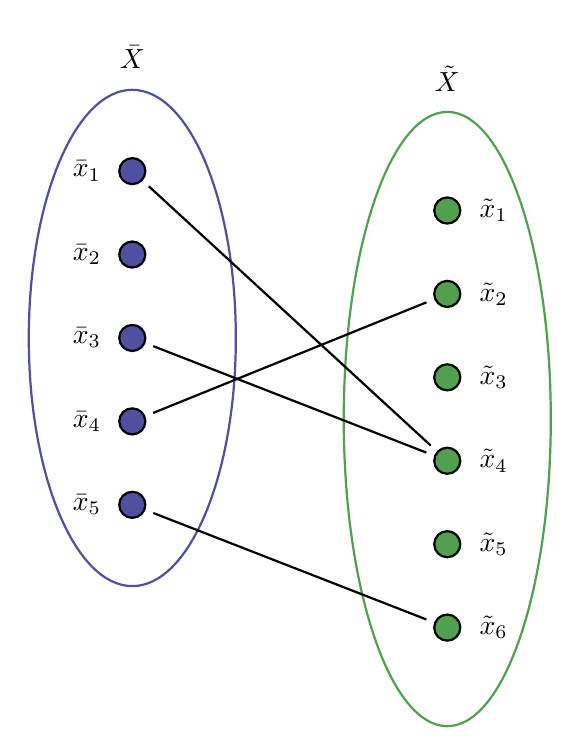
\begin{tikzpicture}[thick,
  every node/.style={draw,circle},
  bnode/.style={fill=myblue},
  tnode/.style={fill=mygreen},
  every fit/.style={ellipse,draw,inner sep=-2pt,text width=2cm},
  ->,shorten >= 3pt,shorten <= 3pt
]

% the vertices of X bar
\begin{scope}[start chain=going below,node distance=7mm]
\foreach \i in {1,2,...,5}
    \node[bnode,on chain, label=left:$\bar{x}_{\i}$] (b\i) {};
\end{scope}

% the vertices of X tilde
\begin{scope}[xshift=4cm,
    yshift=-0.5cm,
    start chain=going below,
    node distance=7mm]
\foreach \i in {1,2,...,6}
    \node[tnode,on chain, label=right:$\tilde{x}_{\i}$] (t\i) {};
\end{scope}

% the set X bar
\node [myblue,fit=(b1) (b5),label=above:$\bar{X}$] {};
% the set X tilde
\node [mygreen,fit=(t1) (t6),label=above:$\tilde{X}$] {};

\draw[-] (b1) -- (t4);
\draw[-] (b3) -- (t4);
\draw[-] (b4) -- (t2);
\draw[-] (b5) -- (t6);
\end{tikzpicture}


    \captionof{figure}{An example of a quasi-bipartite graph on
    \(X~=~\bar{X}~\cup~\tilde{X}\).\\}\label{fig:quasi-example}
\end{minipage}
\begin{minipage}{.75\textwidth}
    \centering
    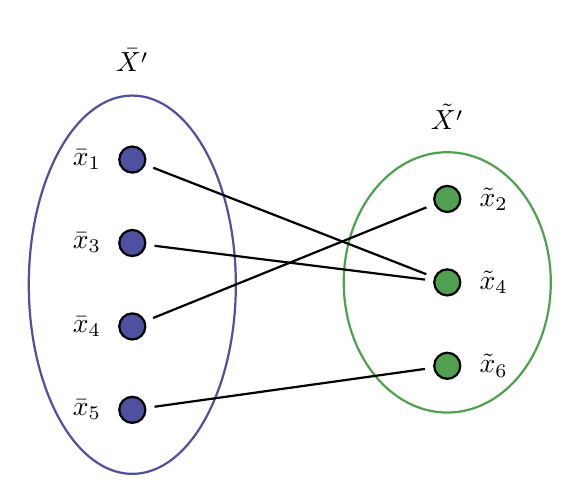
\begin{tikzpicture}[thick,
    every node/.style={draw,circle},
    bnode/.style={fill=myblue},
    tnode/.style={fill=mygreen},
    every fit/.style={ellipse,draw,inner sep=-2pt,text width=2cm},
    ->,shorten >= 3pt, shorten <= 3pt
]

% the vertices of X' bar
\begin{scope}[start chain=going below,
    node distance=7mm
]
\foreach \i in {1, 3, 4, 5}
    \node[bnode, on chain, label=left:$\bar{x}_{\i}$] (b\i) {};
\end{scope}

% the vertices of X' tilde
\begin{scope}[xshift=4cm,
    yshift=-0.5cm,
    start chain=going below,
    node distance=7mm
]
\foreach \i in {2, 4, 6}
    \node[tnode, on chain, label=right:$\tilde{x}_{\i}$] (t\i) {};
\end{scope}

% the set X' bar
\node [myblue, fit=(b1) (b5), label=above:$\bar{X'}$] {};
% the set X' tilde
\node [mygreen, fit=(t2) (t6), label=above:$\tilde{X'}$] {};

\draw[-] (b1) -- (t4);
\draw[-] (b3) -- (t4);
\draw[-] (b4) -- (t2);
\draw[-] (b5) -- (t6);
\end{tikzpicture}

    \captionof{figure}{The bipartite subgraph with vertex sets
    \(\bar{X'}~=~\{\bar{x}_1,~\bar{x}_3,~\bar{x}_4,~\bar{x}_5\}\) and
    \(\tilde{X'}~=~\{\tilde{x}_2,~\tilde{x}_4,~\tilde{x}_6\}\).}
    \label{fig:bipartite-subgraph}
\end{minipage}
\end{figure}

Our objective is to identify and understand the factors which lead to two or
more similar points in our set \(X\) to be split by attribute \(A_m\). With this
formulation, we can achieve this by studying pairs, or subsets, of vertices that
are connected by edges. However, we arrive at a dilemma: the number of pairs to
study requires us to maximise the number of edges \textbf{E} in \(G\), but in
doing so we force the quality of these pairings to be diminished by decreasing
\(\beta\). Ideally, we aim to optimise both of these variables by defining an
objective function in terms of \textbf{E} and \(\beta\) over our set \(X\).

\section{Optimisation problem}\label{sec:optimisation-problem}

For sake of notation let: \(I=|\bar X|, J=|\tilde X|\), a quasi bi-partite graph
\(G=(V, E)\) can be represented by \(A\in \{0, 1\}^{I\times J}\):

\[
    A_{ij}
    =
    \begin{cases}
        1,&\text{ if }(i, j)\in E\\
        0,&\text{ otherwise}
    \end{cases}
\]

A distance matrix \(D\in R(\phi)^{I\times J}\) can be pre computed:

\[
    D_{ij}
    =
    \phi(i, j)
\]

Using, the optimisation problem becomes:

\begin{equation*}
	\begin{aligned}
		& \underset{A}{\text{maximise}}
        &                               & \sum_{ij}A_{ij} \\
        & \text{subject to}
        &                               & A_{ij} \in \{0, 1\} \\
        &
        &                               & A_{ij}\beta \leq D_{ij}
	\end{aligned}
\end{equation*}

Note: this is a standard integer linear program.

% TODO Explore solving with linear solver (see python library: pulp)
% TODO Explore using some stochastic solution that can allow for computation of
% D on the fly

\end{document}
